% ==================================================
% MySQL to Canvas Chart
% Author: Lester James V. Miranda
% ==================================================

\documentclass[preview, convert={outfile=\jobname-out.png,density=300}]{standalone}

\usepackage{tikz}
\usepackage{color}
\usepackage{subfig}
\usepackage{ifthen}
\usepackage{graphicx}
\usepackage{fontawesome}

\renewcommand\familydefault{\sfdefault}

\usetikzlibrary{
    matrix,
    shapes,
    fit,
    arrows,
    positioning,
    calc,
    backgrounds,
    shadows.blur,
    shapes.geometric,
}

\begin{document}
\begin{tikzpicture}[
    node distance = 1cm and 4cm, 
    state/.style={draw, thick, align=center, 
                  minimum width=2cm, minimum height=2cm, 
                  fill=white, text=black, blur shadow={shadow blur steps=5}},
    process/.style={draw, text=black, rounded corners=8pt, 
                    minimum width=2cm, minimum height=0.5cm},
    mycircle/.style={draw=yellow!40, circle, thick, fill=yellow!40, text=black,
                  minimum width=6mm, minimum height=6mm, opacity=0.81},
]

\node[label={[below, yshift=-2cm, align=center]MySQL\\Database}, scale=2] (database) at
    (0,0) {\Huge\faDatabase};

\node[label={[below, yshift=-2cm,
    align=center,name=chartLabel]CanvasJS\\Chart}, scale=2] 
    [right=of database] (chart)
    {\Huge\faAreaChart};

\draw[->, thick] (database) -- (chart)
    node[label={[name=jsonlabel]\faFileO~JSON file}, midway] {};

% STEP 1
\node[mycircle, label={{\color{magenta}\faExclamationCircle}~\color{magenta}AJAX Request}] [above=of chart] (step1) {1};

% STEP 2
\node[mycircle, label={\color{magenta}\faFileCodeO~PHP Service}] [left=of step1, xshift=-1.6cm] (step2) {2};

\draw[->, magenta, dashed, thin] (step1) -- (step2) node [midway, above]
    {\color{magenta}invokes};

% STEP 3
\node[mycircle] at (0,-0.5) (step3) {3};

\draw[->, magenta, dashed, thin] (step2) -- (step3) node
    [midway, right, yshift=0.5cm] {\color{magenta}queries};

% STEP 4
\node[mycircle] [below=of jsonlabel, yshift=0.68cm] (step4) {4};

\draw[->, magenta, dashed, thin] (step3) -- (step4) node[midway,
    below] {\color{magenta}encoded as};

% STEP 5
\node[mycircle] [below=of step1, yshift=-1.18cm] (step5) {5};

\draw[->, magenta, dashed, thin] (step4) -- (step5) node[midway,below,
    xshift=-0.2cm]
    {\color{magenta}rendered as};

%\node[state, label={\textbf{Step 1}}] (AJAXRequest) at (0,0) 
%    {\Large\faExclamationCircle\\AJAX\\ Request \\
%    \texttt{getJSON()}};

%\node[state, label={\textbf{Step 2}}] [right=of AJAXRequest] 
%    (PHPService)
%    {\Large\faFileO\\ PHP\\ Service};


\end{tikzpicture}
\end{document}

